\chapter{Marco Teórico y Estado del Arte}
\ihead[]{Capítulo 2: Marco Teórico y Estado del Arte}
\label{ch:CH02-Estado-del-Arte}
%%%%%%%%%%%%%%%%%%%%%%%%%%%%%%%%%%%%%%%%%%
En este capítulo se presenta una revisión del marco teórico y estado del arte relacionados con la mejora de concentración. Esta revisión tiene como objetivo adquirir los conocimientos fundamentales para el desarrollo conceptual del asistente, estableciendo las bases teóricas que sustentan el presente trabajo.
\section{Marco teórico}
 La presente sección se divide en dos partes: las variables fisiológicas indicadores de concentración y los métodos para mejorar la atención, proporcionando un marco conceptual que orienta el enfoque del asistente.
\subsection{Variables fisiológicas indicadoras de concentración}
%Las variables fisiológicas son  parámetros medibles que permiten regular el buen funcionamiento biológico de un ser vivo. A continuación, se muestran algunas de estas que son capaces de identificar la  concentración en las personas.
\subsubsection{Ondas cerebrales}

Una de las variables fisiológicas que están relacionadas con el estado de concentración y permiten identificar si una persona se encuentra distraída son las ondas cerebrales. Estas son pequeños impulsos eléctricos que las neuronas utilizan para comunicarse entre ellas. Las ondas cerebrales tienen diferente tipo de frecuencia la cual permite clasificarlas en diversos grupos: ondas delta (0.2–4 Hz), theta (4–8 Hz), alfa (8–12 Hz), beta (12–30 Hz) y gamma (30–90 Hz) \autocite{neurofeedback2019}.\\ 

Según \textcite{kaushik2022}, en un estado de concentración, se refleja en un aumento en la amplitud theta en la región parietal izquierda, una disminución en la actividad delta en áreas centrales, y un aumento de amplitud en la actividad Alpha (Figura~\ref{fig:ondas alphfa}) en regiones frontal izquierda. Estos hallazgos sugieren que el análisis de ondas cerebrales permite distinguir entre estados de atención y distracción.
\begin{figure}[H]
\centering
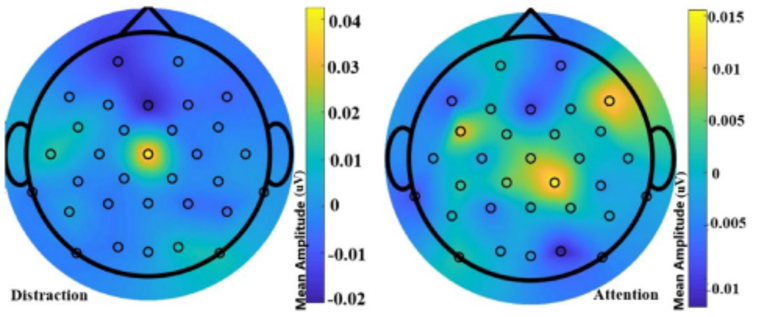
\includegraphics[width=0.7\textwidth]{CHPTRS/CH02_SA/Fig_cap2/Ondas alpha.pdf}
\caption{Amplitudes de las ondas alpha en estado de distracción y atención}
\label{fig:ondas alphfa}
\captionsetup{justification=centering,margin=2cm}
\caption*{\textit{Nota: Figura tomada de Decoding the cognitive states of attention and distraction in a real-life setting using EEG de \linebreak\textcite{kaushik2022}}}
\end{figure}

\subsubsection{Frecuencia cardíaca}
Otra de las variables fisiológicas que pueden estar relacionadas con el estado de concentración es la frecuencia cardíaca. Esta es el número de veces que se contrae el corazón durante un minuto a una determinada presión arterial y frecuencia, la cual oscila entre 50 y 100 latidos por minuto en reposo \autocite{2.frecuencia1}. Uno de las investigaciones realizadas menciona que la variabilidad de frecuencia cardíaca, es decir las fluctuaciones naturales en el tiempo entre los latidos del corazón, en reposo no muestra correlación con el rendimiento de atención en general. Esta variabilidad se asocia con la capacidad de mantener la atención sostenida en tareas prolongadas, a mayor variabilidad, mayor capacidad \autocite{2.frecuencia2}. Asimismo, se ha encontrado que una menor proporción entre los componentes de  \ac{BF} y  \ac{AF} de la variabilidad de frecuencia cardiaca es indicativo de un mejor rendimiento de atención sostenida \autocite{2.frecuencia3}.\\

Por otro lado,  otro estudio determinó que existe la probabilidad de detectar si una persona esta en estado de atención o distracción. En este caso, se tomaron los datos de la frecuencia cardíaca a través de un electrocardiograma conectado a los voluntarios del experimento y los resultados demostraron una precisión de 77\% en la clasificación del estado de atención tras realizar la comparación con los datos obtenidos a través de las ondas cerebrales \autocite{2.electrocardiograma}. 

\subsubsection{Seguimiento ocular}
El seguimiento ocular también es una herramienta que permite identificar los estados de atención o distracción durante el proceso de aprendizaje. Por ejemplo, Alea Bello \textcite{2.clasificacionOcular} presenta una clasificación de niveles de atención: enfocada, selectiva, sostenida, alternada y dividida. En adición a esto, una investigación destaca que la duración total de las fijaciones y el número de fijaciones indican la cantidad de atención asignada así como un procesamiento de información más profundo \autocite{2.ocular2}.

\subsubsection{Señales respiratorias}
Un estudio realizado por \textcite{2.Señalrespiracion1} menciona que las señales respiratorias tienen un gran potencial para el reconocimiento de las emociones, ya que la velocidad y la profundidad de la respiración varían según la emoción humana. Ante carga cognitiva, la frecuencia respiratoria y la ventilación por minuto aumenta durante las tareas cognitivamente demandantes como la concentración \autocite{2.Señalrespiracion2}.\\



\subsection{Métodos para mejorar la atención}
\subsubsection{Técnica Pomodoro}
Una de las técnicas que enfrentan la falta de concentración es la técnica o método Pomodoro. Según el \textcite{2.pomodoro1}, este consiste en dividir las sesiones de estudio en bloques de 25 minutos con la finalidad de alcanzar el foco de concentración. Una vez que se finaliza un bloque, se tiene un descanso de 5 minutos y una vez finalizados los 4 bloques, se tiene un descanso de 20 minutos. Este método tiene una gran cantidad de beneficios como la mejora de concentración, el aumento de la productividad, reducción del estrés, la mejora de la gestión del tiempo, fomenta la disciplina y ayuda a retener información \autocite{2.pomodoro2}.\\

Lo anterior se ve respaldado por un trabajo de investigación realizado por \textcite{2.pomodoro3} sobre el impacto de un aplicativo móvil basada en esta metodología demostró la efectividad de la técnica Pomodoro. En los resultados de dicha investigación, se menciona que el 80\% de los participantes mejoró su nivel de concentración y el 90\% informó que este método ha contribuido a reducir la fatiga durante las sesiones de estudio.

\subsubsection{\textit{Mindfulness}}
Una técnica que ayuda a mejorar la concentración es el \textit{mindfulness}, también conocida como la atención plena o conciencia plena. A pesar de que \textit{mindfulness} no cuenta con una definición única, según  \textcite{2.mindfulness1} y otros autores, coinciden en que se basa en observar la realidad tal como ocurre, aceptándola sin reaccionar impulsivamente. Además, menciona que, como proceso psicológico, implica focalizar la atención en lo que se está haciendo en el aquí y ahora, lo que permite tomar mayor conciencia de las propias acciones y sus consecuencias.\\

Un estudio realizado por \textcite{2.mindfulness2} demostró que la concentración está fuertemente correlacionada con la atención plena, indicando que estas se refuerzan mutuamente. Asimismo, los autores señalan que el mindfulness no solo ayuda la concentración, sino que también promueve estados de tranquilidad, contribuyendo al mejor control atencional que se puede emplear durante actividades académicas o cotidianas.

\subsubsection{Técnica de Respiración consciente}

Otra técnica que permite mejorar la concentración es la respiración consciente. Esta consiste en ser consciente de cada respiración y de la sensación física involucrada en el proceso, lo que permite estabilizar la atención y hacer frente al estrés \autocite{2.Respiracion1}. Un estudio realizado por \textcite{2.Respiracion2} demostró que la práctica de la respiración consciente mejora la atención sostenida, disminuye el estrés y regula el estado emocional de las personas. Estos resultados sugieren que los ejercicios de respiración consciente puede ser una estrategia efectiva para restablecer el enfoque durante periodos de distracción, lo cual resulta útil en el contexto académico.

% NOTA: cada columna tiene un tamaño de x\textwidth, la idea es que la suma de todas las columnas de como máximo 1.
%       Si la suma es mayor a 1, tendras un warning como resultado.
%\begin{longtblr}[theme=pucp,
 %   label = {tab:comparasion-sw},
 %  caption = {Comparacion de \ac{SWA} y \ac{SWB}},
%]{
%    colspec = {X[c,m]X[c,m]X[c,m]},
%    column{1}={0.20\textwidth},
%    column{2}={0.25\textwidth},
%    column{3}={0.25\textwidth},  %este ejemplo 0.3+0.3+.0.2 = 0.8 < 1 (OK!)
 %   rowhead = 1,
 %%   rowfoot = 0,
   % hlines,
   % vlines,
%}
%Característica  & \ac{SWA}        & \ac{SWB} \\
%    Caract. 1   & Descripción A-1 & Descripción B-1\\
%    Caract. 2   & Descripción A-2 & Descripción B-2\\
%    Caract. 3   & Descripción A-3 & Descripción B-3
%\end{longtblr}
%
\section{Estado del Arte}
En esta sección, se mostrarán tanto aquellos dispositivos existentes que permitan recopilar las variables fisiológicas como aquellos que empleen métodos para mejorar la atención. 
    \subsection{\textit{Foci Wearable}}

    El dispositivo FOCI 2 busca aumentar la productividad del usuario a través del monitoreo de su estado cognitivo. Este dispositivo se coloca en la cadera y se calibra en función del patrón de respiración del usuario. En caso de detectar distracción emite una vibración la cual puede ser desactivada mediante su aplicación. A través de dicha aplicación, es posible establecer la duración de la sesión de trabajo profundo que el usuario necesite. A su vez, permite observar las métricas en tiempo real de concentración, fatiga y estrés durante su uso, así como el historial de desempeño del usuario para poder seguir su progreso. El costo del dispositivo es de 100 dólares y viene incluido con su aplicación móvil \autocite{2.foci2025}. Sin embargo, algunos usuarios mencionan que la vibración en la cadera es algo incómoda, por lo que terminan desactivando dicha vibración a través del aplicativo \autocite{2.Foci2}.

  

    
    \begin{figure}[H]
    \centering
    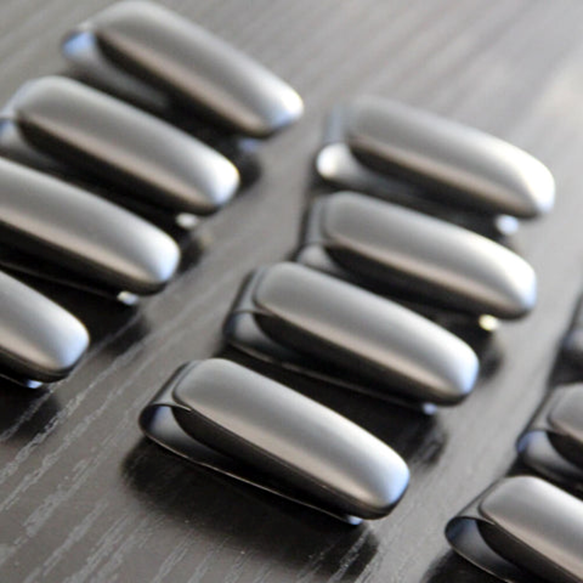
\includegraphics[width=0.3\textwidth]{CHPTRS/CH02_SA/Fig_cap2/Foci.png}
    \caption{Dispositivo FOCI 2}
    \label{fig:foci}
    \caption*{\textit{Nota: Figura tomada de FOCI 2 - Productivity Wearablede  de \linebreak\textcite{2.foci2025}}}
    \end{figure}


  \subsection{\textit{FocusCalm}}
     El dispositivo \textit{FocusCalm} es una vincha inteligente diseñada para medir la actividad eléctrica del cerebro. Su objetivo principal es entrenar la mente a través de diversas actividades de meditación y ejercicios de respiración, a las cuales se accede mediante un aplicativo. Durante el uso, la actividad cerebral se califica de 0 al 100, donde un puntaje bajo refleja niveles elevados de estrés, mientras que un puntaje alto refleja un estado mental de calma. Asimismo, menciona que el uso regular de este dispositivo permite desarrollar un mayor enfoque, disminuir el estrés y una mayor productividad. El precio del dispositivo es de 280 dólares, pero en el aplicativo se tiene que pagar una suscripción única de 170 dólares \autocite{2.focuscalm}.  

    \begin{figure}[H]
    \centering
    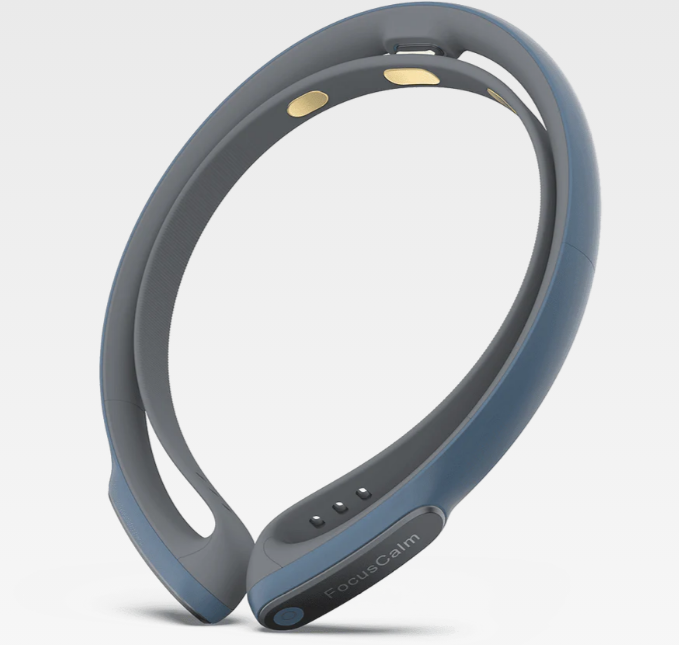
\includegraphics[width=0.2\textwidth]{CHPTRS/CH02_SA/Fig_cap2/FocusCalm.png}
    \caption{Dispositivo \textit{FocusCalm}}
    \label{fig:focus}
    \caption*{\textit{Nota: Figura tomada de FocusCalm EEG Headband de\linebreak\textcite{2.focuscalm}}}
    \end{figure}
    
    \subsection{\textit{Oura Ring 4}}
    El \textit{Oura Ring 4} es un anillo inteligente fabricado con titanio antialergénico, diseñado para el monitoreo fisiológico de quien lo utiliza. Este dispositivo cuenta con sensores discretos que permiten registrar variables como los niveles de oxígeno en la sangre, la frecuencia cardíaca y su variabilidad, la temperatura corporal y los patrones de sueño durante todo el día. Tiene una autonomía de hasta 8 días y cuenta con un aplicativo móvil que ofrece análisis detallados sobre la calidad de sueño, el nivel de estrés, la salud cardiovascular, la actividad física, el ejercicio y, en caso de las mujeres, el seguimiento del ciclo menstrual. El precio del dispositivo es de 350 dólares y para acceder a todas las funcionalidades del aplicativo, se tiene que pagar una supcripción por 70 dólares al año  \autocite{2.OuraRing}.
    
    \begin{figure}[H]
    \centering
    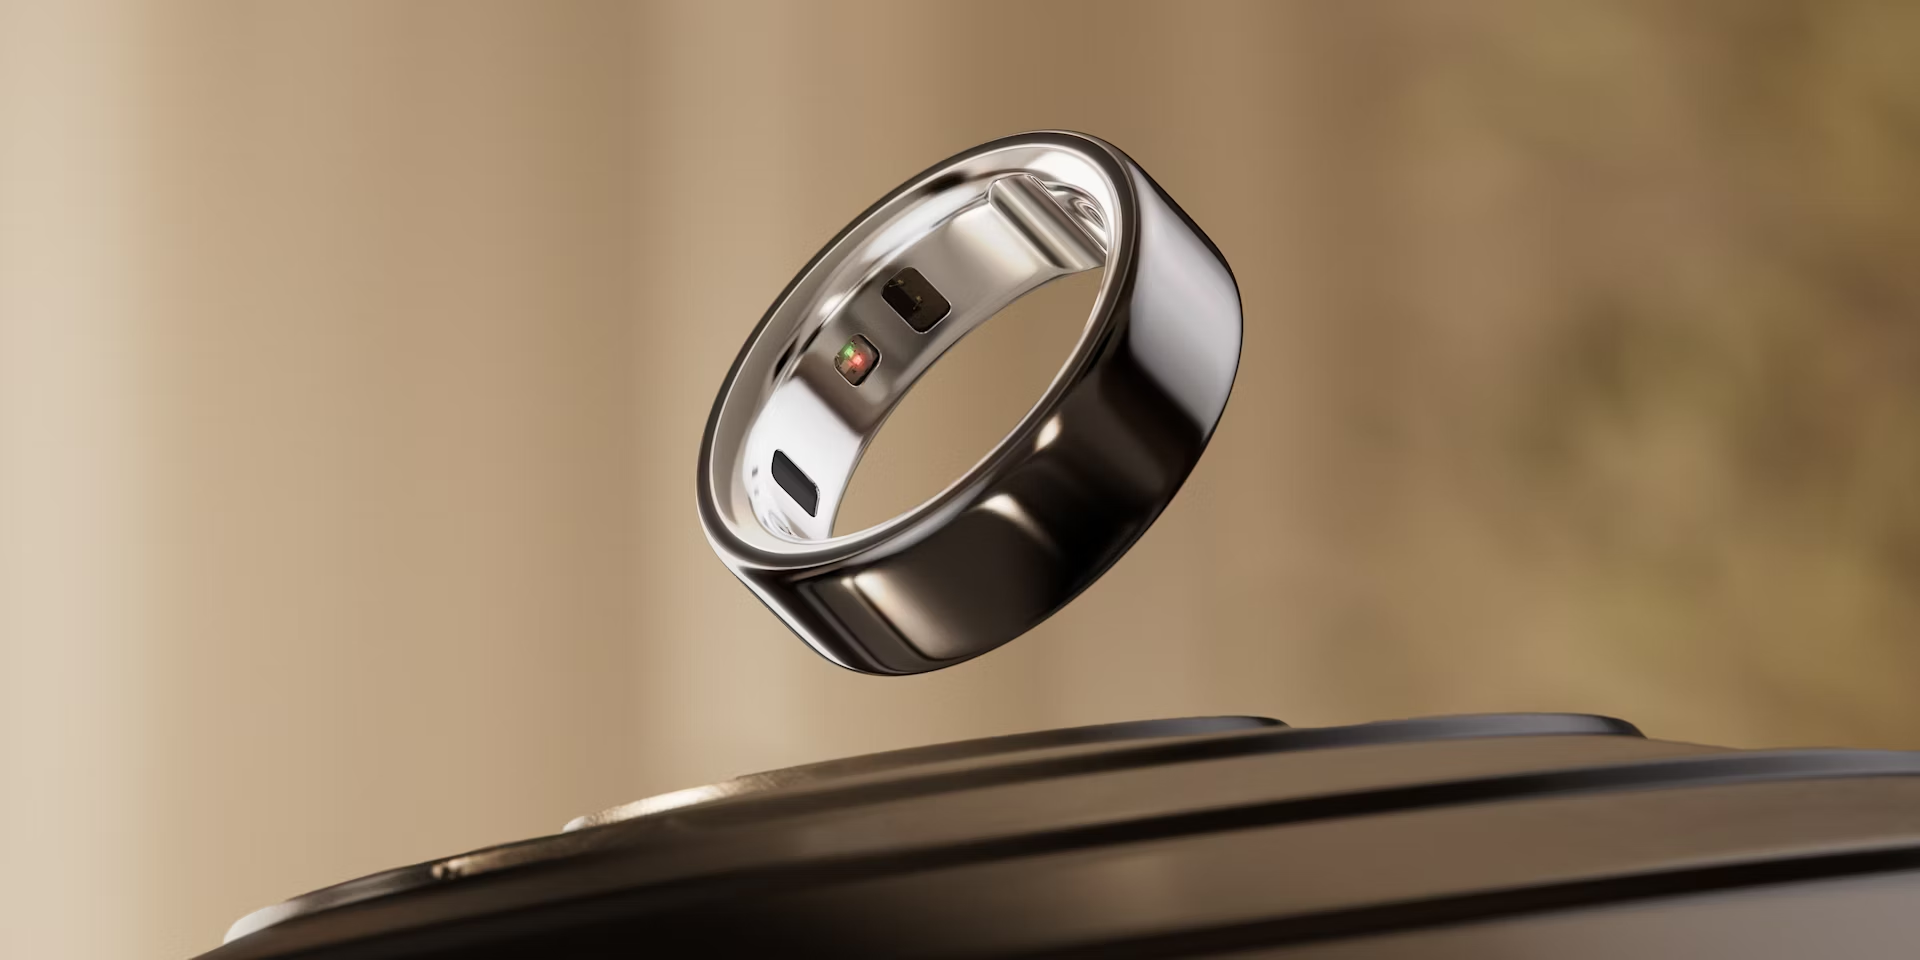
\includegraphics[width=0.3\textwidth]{CHPTRS/CH02_SA/Fig_cap2/Oura.png}
    \caption{Dispositivo \textit{Oura Ring 4}}
    \label{fig:oura}
    \caption*{\textit{Nota: Figura tomada de Oura Ring 4: Nuestro anillo inteligente más sofisticado de\linebreak\textcite{2.OuraRing}}}
    \end{figure}
    
\subsection{Comparación de dispositivos}
En la siguiente Tabla ~\ref{tab:Tabla Comparativa entre Dispositivos} se hace la comparación entre los dispositivos mencionados previamente. Para ello, se determinó ciertos aspectos importantes como retroalimentación, forma, característica principal y precios.

\begin{table}[H]
        \centering
        \caption{Tabla comparativa entre dispositivos}
        \label{tab:Tabla Comparativa entre Dispositivos}
        \begin{tblr}{
          width = \linewidth,
           colspec = {X[c,m] X[c,m] X[c,m] X[c,m]},
            %column{1}={0.2\textwidth},
            %column{2}={0.2\textwidth},
            %column{3}={0.2\textwidth},
            %column{4}={0.25\textwidth},
          cells = {c},
          hlines,
          vlines,
          hline{1,7} = {-}{0.08em},
        }
        Nombre                       & Foci Wearable~ ~                               & FocusCalm                             & Oura Ring 4                                                                     \\
        Precio Unitario              & \textbf{\$}130                                 & \textbf{\$}279.99                     & \textbf{\$}349                                                                  \\
        Precio de suscripción        & Incluido con el dispositvo                     & \textbf{\$}169.99 (pago unico)        & \textbf{\$}69.99 por año                                                        \\
        {Característica \\principal} & {Medición del \\patron respiratorio}           & {Medición de \\ondas cerebrales~~}    & {Medición de frecuencia cardiaca, \\niveles de oxigeno y temperatura corporal~} \\
        Retroalimentación            & {Vibración y estadísticas \\por el aplicativo} & {~ ~Estadísticas \\por el aplicativo} & {~ Estadísticas \\por el aplicativo}                                                 \\
        Forma                        & Clip compacto                                  & Vincha                                & Anillo                                                                          
\end{tblr}
\end{table}
   % \begin{table}[H]
    %    \centering
        
     %   \caption{Parámetros Máquina 1 (modelo 80085). Ver paquete \url{https://ctan.org/pkg/siunitx}}
      %  \begin{tblr}{
       %%%     cell{3}{3} = {c},
        %      cell{4}{3} = {c},
         %     cell{5}{3} = {c},
        %}
    %    \hline
    %    Características & Valor          &  \\
    %    \hline
    %    Param. físico 1 & \SI{4.1}{\ohm} &  \\
    %    Param. físico 2 & \SI{0.14}{\mH} &  \\
    %    Param. físico 3 & ... &  \\
    %    Param. físico 4 & ... &  \\
    %    Param. físico 5 & ... &  \\
    %    Param. físico 6 & ... &  \\
    %    Param. físico 7 & ... &
   %     \end{tblr}
  %      \caption*{\small\textit{Nota: Información adaptada de xxxx ..., revisada el día DD de MM de AAAA.\autocite{ej-03-cita-pag-web}}} %revisada el día 25 de setiembre del 2024}
 %       \label{tab:ejemplo_tabla_con_unidades}
%    \end{table}



  
   